\documentclass[../catalog.tex]{subfiles}

\begin{document}

\subsubsection{Problem}

Throughout the previous chapters we have seen how delta queries and
worst-case optimal join algorithms make much of 3DF's design
possible. We have arrived at a system that provides robust,
predictable performance within a multi-user environment, at high
throughputs, with low latencies, and with bounded memory use. In doing
so, we have overcorrected a bit, at the expense of redundancies in the
overall dataflow. Apart from the attribute indices, we have foregone
almost all opportunities for sharing state between dataflows.

Query dataflows consume a number of ressources over their entire
lifetime, which might be measured in minutes or hours for interactive
sessions, but in days, weeks, months, or even years for dataflows
between backend services.

[@TODO overheads of dataflow elements]

Naturally, this limits the number of clients we can support
concurrently.

\subsubsection{Example}

[@TODO analyst queries]

Consider again a scenario of many analysts concurrently interacting
with the same data streams. Many of them will be interested in a
common subset of data, e.g. users that are currently active in Europe,
but will impose some additional constraints depending on their
respective tasks at hand.

\texttt{@TODO example: shared access policy?}

A more concrete example might be the comment stream from previous
chapters:

\begin{verbatim}
[(comment ?comment ?place ?person ?ip ?content \ldots{})

 [?comment :comment/creation-date ?creationDate]
 [?comment :comment/creator ?person]
 [?comment :comment/ip ?ip]
 [?comment :comment/browser ?browser]
 [?comment :comment/content ?content]
 [?comment :comment/place ?place]]
\end{verbatim}

We have multiple analysts, each interested only in comments from a
specific location. For an analyst interested in comments originating
in Zurich, a query might look like the following:

\begin{verbatim}
[:find \ldots{}
 :where
 (comment ?comment ?place \ldots{})
 [?place :place/name "Zurich"]]
\end{verbatim}

Given $n$ analysts, we can service their queries in three different
ways.

\subsubsection{Shared Nothing}

We create $n$ indepedent dataflows, sharing only the base
relations. This gives us the greatest freedom to pick the best
possible plans for each individual analyst, for example making use of
the worst-case optimal join framework introduced in chapter
\texttt{@TODO}.

On the other hand, all of those $n$ dataflows will perform a lot of
redundant work and incur significant overheads, essentially derivingq
$n$ copies of the \texttt{comment} relation. Dataflow elements are not
free either, and will incur scheduling and other bookkeeping
overheads.

Computing multiple redundant instance of a plan where worst-case
optimal execution improves the asymptotic complexity can still be
significantly cheaper.

\subsubsection{Shared Trunk}

Differential's \emph{arrangements} allow us to re-use materialized
relations between dataflows. We could therefore create a single
dataflow deriving the \texttt{comment} relation, on top of which $n$
specialized dataflows will be only be responsible for implementing the
specific additional joins requested by each analyst. Because
arrangements materialize tuples into sorted batches, doing so will
cost extra storage proportional in the size of the `comment` relation,
on top of the storage taken up by base relations
(c.f. \ref{case-join-state}).

Sharing a common part of the dataflow (a \emph{shared trunk}) avoids
redundant derivations of the \texttt{comment} relation and
significantly reduces the total number of dataflow elements created (a
super-linear reduction in case of delta-queries), at the cost of some
extra storage — seemingly a fine trade-off!

On the other hand, materializing a shared trunk fixes the space of its
possible implementations. In particular (as touched on in
\ref{case-eagerness}) it prevents us from exploiting highly selective
constraints provided by individual analysts to cut down on the number
of tuples produced by each flow.

In the specific case of the \texttt{comment} relation, this might not
be a problem, as the number of tuples produced during its derivation
is proportional to the number of comments in the system. For other
relations (for example the transitive graph induced by the
\texttt{:person/knows} relation) it might lead to catastrophic plans.

Whenever we are considering to build multiple dataflows off of a
shared trunk, we must therefore estimate whether the shared trunk is
\emph{sufficiently constrained}. This brings us back to the problem
initially observed in \ref{case-eagerness}. After all our work to
avoid heuristics and cardinality estimation, this would re-introduce
an element of unpredictability into the behaviour of our system.

Additionally, once we've made the decision to share a flow, we must
commit to maintaining it for as long as any dependent flows are
active. Sharing via arrangements, in the current implementation, also
causes some subtle coupling that can cause problems, if dependent
dataflows don't make progress at roughly the same pace:

\begin{quote}
[\ldots{}] by sharing the data we also need to share the restrictions
we impose on the data when it comes to compaction of the history. If
we have some operator that is failing to move forward in time, or
doing so slowly, it may require the trace maintain historical data
that others do not need so that it can operate correctly. Other
operators will have to flip through historical distinctions that they
themselves wouldn't have maintained, and could execute less
efficiently than if they had their own personally compacted
representation.

\cite{makingarrangements}
\end{quote}

\subsubsection{Multi-Tenant Dataflows}

Luckily, an additional implementation strategy is available to us: we
can model multi-tenancy within the data plane itself. Recall the query
from earlier:

\begin{verbatim}
[:find \ldots{}
 :where
 (comment ?comment ?place \ldots{})
 [?place :place/name "Zurich"]]
\end{verbatim}

As a first step, we will re-write this query, replacing the explicit
filter by a parameter input, drawn from an additional parameter
attribute.

\begin{verbatim}
[:find \ldots{}
 :where
 (comment ?comment ?place \ldots{})
 [?place :place/name ?name-filter]
 [\_ :parameter/place-name ?name-filter]]
\end{verbatim}

This is useful in an of itself, because it gives us the ability to
update the filter parameter (with updated results derived
incrementally as usual), without registering separate queries.

It takes only a few extensions to generalize this approch to multiple
concurrent users.

First, we must indicate to 3DF, that the
\texttt{:parameter/place-name} attribute adheres to special
semantics. In particular, we must enforce, that clients may only add
or retract values to it, they can not control the keys. Where usually
a transaction would take the form \texttt{[:db/add <eid>
    :parameter/place-name <value>]}, 3DF will only allow
\texttt{[:db/add :parameter/place-name <value>]}.

Rather, for all updates from a specific client, we will automatically
associate that client's connection token as the key. This way, we can
distinguish between parameters from different client. We make use of
this information to route results correctly to their respective
clients.

This allows us to use a single dataflow for all $n$ analysts, while
still being able to move the `:place/name` constraints into the same,
worst-case optimal query plan.

We find precedence for this approach in the NiagaraCQ system by
\cite{chen2000niagaracq}.

\begin{quote}
NiagaraCQ implements sharing even when operators differn in certain
constants, by implementing the operators using relational joins
against the table of constants \cite{chen2000niagaracq}.

\cite{hirzel2014catalog}
\end{quote}

\subsubsection{Other Strategies}

Again from \cite{hirzel2014catalog} we learn that

\begin{quote}
YFilter implements sharing between applications written in a subset of
XPath by compiling them all into a combined NFA [Diao et al. 2002].
\end{quote}

Similar NFA-based approaches can be found in the literature on complex
event processing (e.g. \cite{agrawal2008}). While such methods are
available to us in Timely Dataflow (e.g. via the built-in
`StateMachine` operator), they do not fit cleanly into the relational
model implemented by 3DF and Differential Dataflow. The question of
whether the two approaches can be combined in a sensible way is left
for future inquiry.

\subsubsection{Identifying Opportunities For Sharing}

Finding common sub-structures across query plans that would be
suitable for either of the approaches outlined above is in general a
very computationally intensive problem. For the purposes of this work
we will not consider arbitrary re-use across rules, but rather stick
to the following simplified approach.

3DF already enforces that each registered rule be given a unique
name. We can further break this down and give unique names to all
conjunctions, e.g. by creating separate rules for the different
branches of an `or` clause automatically.

Additionally, we can split off plan stages that do not affect the
underlying joins, such as `Transform` and `Aggregate`.

\texttt{@TODO}

\subsubsection{Remedy}

Here we are meeting again a trade-off identified in the very first
scenario we analysed, \texttt{Case 0}.

\subsubsection{Evaluation}

\begin{figure}[h!]
  \begin{subfigure}{.5\textwidth}
    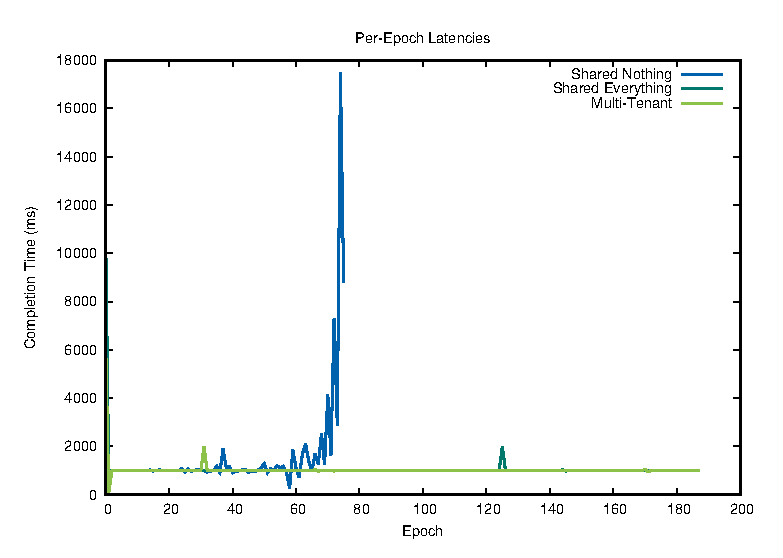
\includegraphics[width=1.0\linewidth]{results/multitenant_w1_p1/times}
    \caption{Single Worker}
  \end{subfigure}
  \begin{subfigure}{.5\textwidth}
    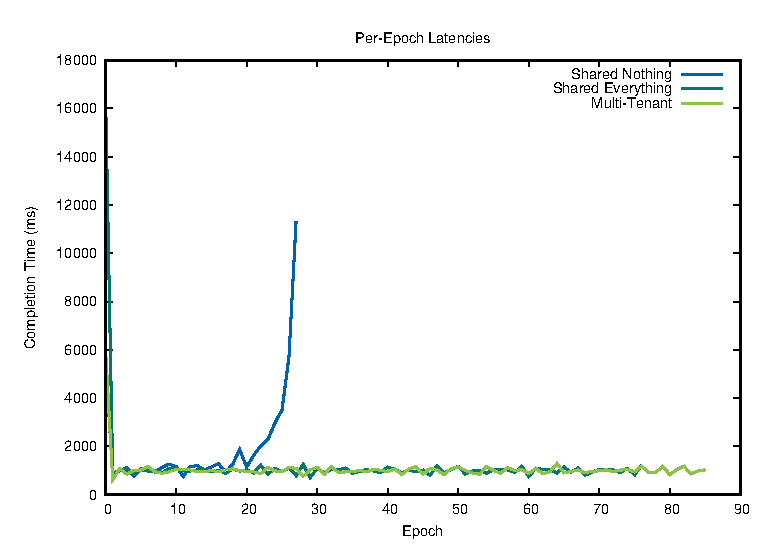
\includegraphics[width=1.0\linewidth]{results/multitenant_w1_p3/times}
    \caption{Three Distributed Workers}
  \end{subfigure}

  \caption{Per-Epoch Latencies}
\end{figure}

\subsubsection{Future Work}

We think that expressing multi-tenancy within the data plane is a very
powerful implementation strategy for dataflow systems. Still we might
think about different ways to accomplish the same goal. Recall that we
kept track of what parameters were associated with which client via
the keys of a parameter relation.

This approach has drawbacks when overlap between parameters from
different tenants is high.

In such cases we could make use of the fact, that sets of client
tokens form a commutative monoid under set union. Any such monoid can
take the place of Differential's multiplicities (and benefit from
efficient in-place updates).

@TODO
If we want to re-use delta query pipelines we might have to generalize
~AltNeu~ to be an integer, specifying the position in the
chain. Otherwise the likelihood of compatible re-use across pipelines
is negligible.

@TODO iterated hector
There is a remaining redundancy in Hector, in that whenever multiple
Attribute bindings refer to the same attribute, we would be
constructing more than one delta pipeline. In a way, a single change
to the supporting attribute leads to multiple changes in the bindings.

\end{document}
